\documentclass[conference]{IEEEtran}
\usepackage{amsmath,amssymb}
\usepackage{booktabs,array}
\usepackage{graphicx}
\usepackage{tikz}
\usetikzlibrary{arrows.meta,positioning,fit,backgrounds}
\usepackage{cite}
\usepackage{url}
\usepackage[hidelinks]{hyperref}
\usepackage{balance}


\newcommand{\etal}{\textit{et al.}}
\newcommand{\ie}{\textit{i.e.}}
\newcommand{\eg}{\textit{e.g.}}
\newcommand{\viz}{\textit{viz.}}
\newcommand*{\email}[1]
{\normalsize\texttt{\href{mailto:#1}{#1}}\par}

\newcommand{\Bhat}{\widehat{B}}
\newcommand{\ind}{\mathbf{1}}
\newcommand{\Normal}{\mathcal{N}}
\newcommand{\Ttwo}{T_2^{\ast}}
\newtheorem{lemma}{Lemma}
\newtheorem{proposition}{Proposition}
\newtheorem{corollary}{Corollary}
\newtheorem{theorem}{Theorem}
% Generated from audited frozen confirmation; do not edit numbers by hand.
\newcommand{\TotalN}{15{,}360}
\newcommand{\NominalHarmCount}{3{,}192}
\newcommand{\NominalHarmRate}{20.78}
\newcommand{\NominalHarmCI}{20.26, 21.30}
\newcommand{\SmallHarmCount}{11{,}510}
\newcommand{\SmallHarmRate}{74.93}
\newcommand{\SmallHarmCI}{74.08, 75.83}
\newcommand{\WeakHarmRate}{99.76}
\newcommand{\WeakReferenceHarmRate}{62.25}
\newcommand{\FallbackCleanRMSE}{6.14}
\newcommand{\ReferenceCleanRMSE}{19.98}
\newcommand{\FallbackAttackRMSE}{23.21}
\newcommand{\ReferenceAttackRMSE}{19.96}
\newcommand{\CleanAlarmRate}{1.07}
\newcommand{\CleanAlarmCI}{0.91, 1.24}
\newcommand{\AbstainAttackN}{296}
\newcommand{\AbstainAttackH}{296}
\newcommand{\AbstainAttackCoverage}{1.93}
\newcommand{\AbstainAttackRisk}{100.00}
\newcommand{\AbstainShotsMillions}{1.04}
\newcommand{\PrimaryHarm}{296}
\newcommand{\ReferenceHarm}{2{,}896}
\newcommand{\GenuineAlarmCount}{154}
\newcommand{\MismatchAlarmRate}{7.68}
\newcommand{\MismatchHarmRate}{1.88}
\newcommand{\HalfHarmRate}{89.67}
\newcommand{\FullHarmRate}{99.98}
\newcommand{\FullAlarmRate}{0.94}
\newcommand{\RunMinutes}{75.6}
\newcommand{\StoredTestCount}{614{,}400}
\newcommand{\StoredCalibrationCount}{737{,}280}
\newcommand{\ArchiveMB}{349.7}
\newcommand{\VerifiedArtifacts}{3{,}213}
\newcommand{\AttackerEvals}{90{,}000}
\newcommand{\SearchStarts}{120}
\newcommand{\EquivalenceError}{5.55\times 10^{-16}}
\newcommand{\FixedU}{14{,}758}
\newcommand{\HiddenU}{1}
\newcommand{\FrequencyU}{14{,}892}
\newcommand{\OptimizedT}{6{,}081}
\newcommand{\OptimizedU}{17}
\newcommand{\MeanU}{14}
\newcommand{\CleanDifference}{-13.84}
\newcommand{\CleanDifferenceCI}{-14.27, -13.44}
\newcommand{\PrecisionStatement}{The predefined precision goals were all met; the fixed run was not extended.}

% Generated by analysis/project1/reference_theory.py. Theory*/Spin* values are
% post-hoc models, not endpoints; Obs* values are replayed or quoted results.
\newcommand{\ObsPFourDiff}{18.85}
\newcommand{\ObsPFiveDiff}{98.07}
\newcommand{\ObsBiasHarmRate}{26.94}
\newcommand{\ObsIVWClean}{4.29}
\newcommand{\ObsIVWAttack}{100.00}
\newcommand{\TheoryKappaGap}{0.6}
\newcommand{\TheoryMaxGap}{0.60}
\newcommand{\TheoryConditions}{8}
\newcommand{\TheoryAbstainPred}{1.74}
\newcommand{\TheoryAbstainObs}{1.93}
\newcommand{\TheoryKappaTwenty}{57.6}
\newcommand{\TheoryBlindUpper}{32.6}
\newcommand{\TheoryFloorUpper}{82.6}
\newcommand{\TheoryZ}{2.807}
\newcommand{\TheorySigmaPrimary}{4.28}
\newcommand{\TheorySigmaCritical}{17.3}
\newcommand{\TheoryFloorTwenty}{21.13}
\newcommand{\TheoryAvgReadings}{11}
\newcommand{\TheoryAvgSigma}{6.03}
\newcommand{\TheoryAvgFloor}{0.003}
\newcommand{\SpinMaxDiff}{4.8}
\newcommand{\SpinSignal}{0.034}
\newcommand{\SpinShotNoise}{0.016}
\newcommand{\TheoryNearFive}{0.1}
\newcommand{\TheoryNearFifteen}{77.3}
\newcommand{\TheoryNearTwenty}{97.7}
\newcommand{\TheoryNearFifty}{100.0}

\title{When the Sensor Cannot Tell: Control Spoofing and the Limits of
Reference Fallback in NV Ramsey Magnetometry}
\author{
    \IEEEauthorblockN{%
         Sounak Bhowmik and
         Himanshu Thapliyal 
                    }
 
    \IEEEauthorblockA{Department of Electrical and Computer Engineering\\
        Southern Methodist University, Dallas, TX, USA}
    \email{sbhowmik@smu.edu},
    \email{hthapliyal@smu.edu}            
}

\begin{document}
\maketitle

\begin{abstract}
In Ramsey magnetometry, magnetic field estimation relies on a quantum phase shift that is inherently coupled to the microwave control drive. We investigate what a defender can detect and recover when an adversary manipulates the drive of a nitrogen-vacancy (NV) transition. Because a drive-frequency offset is physically indistinguishable from a true field shift under arbitrary pulse shapes and interrogation schedules, the sensor cannot independently verify its own readings. While randomized interrogation timing mitigates phase attacks bound to a public schedule, full spoof detection necessitates an independent reference sensor. We prove that, under a harmful spoof attack, falling back to an auxiliary reference upon alarm yields no accuracy advantage over relying solely on the reference. Furthermore, within a location model, no translation-equivariant fusion or output rule can beat the reference's error floor under worst-case spoof magnitude. We derive a closed-form expression predicting the residual harm and identifying a ``blind window'' of small yet harmful spoofs. A pre-registered, frozen simulation campaign across 30 seeded pipeline replicates validates these theoretical limits: with a 20~nT reference, fallback releases harmful estimates on \NominalHarmRate\% of 100~nT spoofs—matching the error rate of the standalone reference. Crucially, these guarantees hold only if the reference sensor shares no clock, microwave synthesizer, or data path with the primary system.
\end{abstract}

\begin{IEEEkeywords}
NV magnetometry, Ramsey sensing, sensor spoofing, control integrity,
identifiability, reference-assisted verification
\end{IEEEkeywords}

% ======================================================================
\section{Introduction}
\label{sec:intro}

Nitrogen-vacancy (NV) magnetometers are promising candidates for field deployment~\cite{barry2020sensitivity}, such as in magnetic anomaly navigation where measured fields map directly to spatial coordinates~\cite{canciani2016magnav}. In these applications, field estimation errors propagate directly into navigation errors. While the quantum state itself is inherently resistant to remote manipulation, its supporting classical control hardware is far more vulnerable. Microwave synthesizers, arbitrary waveform generators, and shared clock sources establish the phase frame for Ramsey sequences, while analog control lines remain susceptible to signal injection~\cite{kune2013ghost,shoukry2013abs}. This motivates a fundamental security question: \emph{If an attacker manipulates the microwave control drive of an NV Ramsey magnetometer, what can a defender detect, and to what extent can the field estimate be recovered?}

The answer turns on one fundamental physical identity: along a single transition, a microwave drive-frequency detuning enters the Ramsey phase equation identically to a Zeeman shift. Consequently, an adversary can perfectly spoof the measurement statistics of an arbitrary target field. No internal anomaly detector, machine learning model, or secret timing schedule can distinguish spoofed counts from legitimate field shifts using the primary sensor's data alone. Detection must therefore rely on an auxiliary reference sensor. A common architectural response is to trigger an alarm when the primary and reference sensors diverge, falling back to the reference measurement. However, evaluating such architectures purely by detection probability is misleading for field estimation: once the primary sensor is compromised, any accurate output depends entirely on the reference channel.

\textbf{Contributions:} While undetectable physical attacks are well studied in cyber-physical systems~\cite{pasqualetti2013attack} and detuning--field equivalence is grounded in quantum physics, our primary contribution lies in characterizing the fundamental recovery limits across concrete Ramsey actuation models:
\begin{enumerate}
\item \textbf{Fundamental Identifiability Analysis} (Section~\ref{sec:identifiability}): We show that microwave drive detuning is mathematically equivalent to a Zeeman field shift for arbitrary rotating-frame dynamics. A full lab-frame spin-1 simulation bounds unaddressed transition residuals. We establish that secret interrogation timing defends only against committed phase attacks, whereas dual-transition schemes force two-tone manipulation.
\item \textbf{Theoretical Recovery Limits} (Section~\ref{sec:reference}): We prove that fallback policies cannot exceed the accuracy of the standalone reference during a harmful spoof (Proposition~\ref{prop:bound}). Within a location-estimation model, no translation-equivariant rule can bypass the reference's error floor in the worst case (Theorem~\ref{thm:floor}). We derive closed-form expressions for the residual harm, define a critical ``blind window,'' and establish reference precision requirements.
\item \textbf{Pre-Registered Confirmation and Fusion Analysis} (Sections~\ref{sec:design}--\ref{sec:results}): Using 30 independently seeded simulation pipelines under a pre-registered protocol, we validate these theoretical bounds. Post-hoc analysis shows our closed-form predictions accurately match all \TheoryConditions{} simulated reference conditions, illustrating how estimation precision trades off against worst-case integrity across fusion strategies.
\end{enumerate}

\textbf{Scope and Organization.} Our results are grounded in theoretical analysis and numerical simulation.
% ; physical hardware validation remains future work. 
We assume the attacker manipulates only the primary microwave drive and that the reference operates as an independent sensing channel. This independence assumption is deployment-critical: any reference sharing a clock, synthesizer, or hardware interface with the primary sensor fails under identical attacks (Section~\ref{sec:threat}). The remainder of this paper is organized as follows: Section~\ref{sec:threat} presents the system and threat model; Section~\ref{sec:identifiability} analyzes sensor identifiability limits; Section~\ref{sec:reference} proves limits on reference-assisted recovery; and Sections~\ref{sec:design}--\ref{sec:discussion} present the confirmation protocol, experimental findings, and system implications.

% ======================================================================
\section{System and Threat Model}
\label{sec:threat}

Fig.~\ref{fig:pipeline} illustrates the architecture and the trust boundaries. A trusted scheduler selects interrogation durations $t_k$ and analysis phases $\phi_k$, logging them in a tamper-proof command record. A downstream control hardware path converts these commands into microwave pulses addressing a single NV transition. The estimator reconstructs the magnetic field from observed photon counts and logged commands, while a verification module computes scores on held-out interrogation data. An optional reference sensor provides an independent field measurement $R$ via a separate signal path.

\begin{figure*}[t]
\centering
% Native TikZ source: no external renderer or shell-escape required.
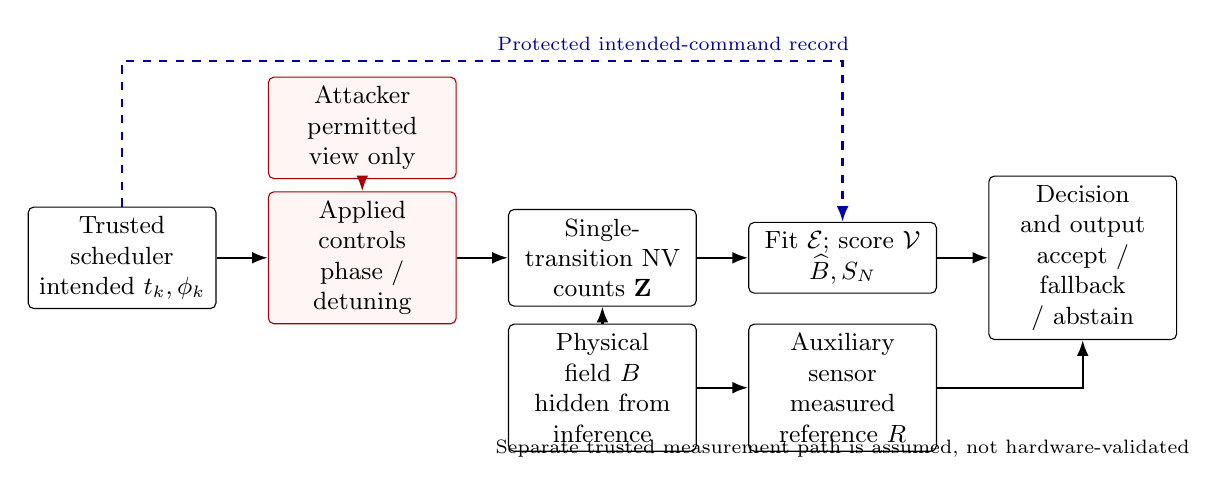
\begin{tikzpicture}[
  block/.style={draw,rounded corners=2pt,align=center,font=\small,
                minimum height=0.85cm,text width=2.15cm,fill=white},
  flow/.style={-{Latex[length=2mm]},thick},
  metadata/.style={flow,dashed,blue!65!black},
  note/.style={font=\scriptsize,align=center},
  x=1cm,y=1cm]
\node[block] (scheduler) at (0,0) {Trusted scheduler\\intended $t_k,\phi_k$};
\node[block,draw=red!65!black,fill=red!4] (control) at (3.05,0)
  {Applied controls\\phase / detuning};
\node[block] (sensor) at (6.1,0) {Single-transition NV\\counts $\mathbf Z$};
\node[block] (inference) at (9.15,0) {Fit $\mathcal E$; score $\mathcal V$\\$\widehat B, S_N$};
\node[block] (decision) at (12.2,0) {Decision and output\\accept / fallback / abstain};
\node[block,draw=red!65!black,fill=red!4] (attacker) at (3.05,1.65)
  {Attacker\\permitted view only};
\node[block] (field) at (6.1,-1.65) {Physical field $B$\\hidden from inference};
\node[block] (reference) at (9.15,-1.65) {Auxiliary sensor\\measured reference $R$};
\draw[flow] (scheduler) -- (control);
\draw[flow] (control) -- (sensor);
\draw[flow] (sensor) -- (inference);
\draw[flow] (inference) -- (decision);
\draw[flow,red!65!black] (attacker) -- (control);
\draw[flow] (field) -- (sensor);
\draw[flow] (field) -- (reference);
\draw[flow] (reference.east) -| (decision.south);
\draw[metadata] (scheduler.north) -- (0,2.5) -- (9.15,2.5) -- (inference.north);
\node[note,text=blue!65!black] at (7,2.72) {Protected intended-command record};
\node[note] at (9.15,-2.43) {Separate trusted measurement path is assumed, not hardware-validated};
\end{tikzpicture}

\caption{System and trust boundaries. The attacker alters applied controls after command generation; the intended-command record (blue, dashed) stays protected. The reference path is assumed to lie outside attacker control. True field, applied-control logs and attack labels are used only for evaluation.}
\label{fig:pipeline}
\end{figure*}

\textbf{Assets and Security Endpoints.} The primary security asset is the integrity of the released field estimate $Y$. Table~\ref{tab:metrics} formalizes the evaluation metrics. An output release is classified as \emph{harmful} if $|Y-B| > \epsilon_H = 25$~nT. System availability is evaluated separately, as trivially suppressing all outputs prevents harm but negates utility. The attacker's goal is to inject a target offset $\Delta B$, forcing an unalarmed release within $\epsilon_T = 10$~nT of $B+\Delta B$. Both threshold tolerances ($\epsilon_H, \epsilon_T$) are experimental parameters chosen for rigorous benchmark evaluation rather than rigid operational standards.

\begin{table}[t]
\centering
\caption{Endpoints, per condition over $n$ attempts. $L_i=1$ if attempt $i$ releases an output $Y_i$; $A$ is the alarm.}
\label{tab:metrics}
\footnotesize
\begin{tabular}{@{}lp{0.64\columnwidth}@{}}
\toprule
Endpoint & Definition \\
\midrule
Harm $H$ & $1/n\sum_i L_i\ind\{|Y_i-B_i|>\epsilon_H\}$, per attempt \\
Coverage $C$ & $1/n\sum_i L_i$, fraction of outputs released \\
Selective risk $Q$ & $H/C$, harm among releases (undefined if $C=0$) \\
Undetected success $U$ & $\ind\{|\Bhat-(B+\Delta B)|\le\epsilon_T\}(1-A)$ \\
RMSE & root mean squared error over released outputs \\
\bottomrule
\end{tabular}
\end{table}

\textbf{Adversary Capability Model.} The adversary manipulates the microwave drive addressing the target NV transition using one of two physical actuation channels: an analysis-phase offset or a constant drive-frequency detuning. We evaluate four information profiles reflecting the adversary's prior knowledge:
\begin{itemize}
\item \textbf{A0}: Operates without schedule information.
\item \textbf{A1}: Knows the public, nominal schedule.
\item \textbf{A2}: Observes the actual challenge sequence only if disclosed before a $2\,\mu\text{s}$ actuation deadline.
\item \textbf{A3}: Obtains immediate, real-time knowledge of interrogation challenges.
\end{itemize}
The adversary cannot observe the true ambient field $B$, defender calibration parameters, or reference measurements, nor can it tamper with optical readout data, command logs, downstream inference software, or the reference hardware path.

These boundaries explicitly delineate the security scope. An adversary capable of modifying photon counts, command logs, or estimation software directly controls system output, bypassing statistical verification entirely; mitigating such threats requires cryptographic data-path protection. Similarly, compromising the reference path reduces to our fully shared dependency case. We do not model adaptive spoofing across sequences, multi-actuator co-optimization, or calibration poisoning. Consequently, our findings represent fundamental physical recovery limits against drive manipulation rather than guarantees against broader system compromises.

Manipulating the drive frequency requires remarkably low effort. Synthesizing a $100\text{~nT}$ spoof corresponds to a frequency offset of $\gamma\Delta B / 2\pi = 2.8\text{~kHz}$—roughly $1\text{~ppm}$ of the $2.87\text{~GHz}$ carrier frequency. Because microwave synthesizers lock to a $10\text{~MHz}$ reference clock, a $1\text{~ppm}$ clock drift or external clock pulling produces an identical shift. This falls well within standard crystal oscillator tolerances, implying that an uncalibrated or shared clock introduces systematic field bias. A secondary NV sensor sharing the master clock inherits this identical offset.

\textbf{Trust Assumptions.} System security relies on a trustworthy initialization state: clean initial calibration, stored error models, decision thresholds, scheduling routines, and inference algorithms are all trusted. The reference channel is modeled as an abstract signal $R = B + \text{noise}$ operating outside the attack graph.

\textbf{Deployment-Critical Assumption: Reference Independence.} All recovery guarantees established herein require a reference channel completely isolated from drive manipulation. Table~\ref{tab:audit} maps common shared hardware dependencies to their analytical parameters and experimental stress cases. A fully shared reference renders anomaly detection virtually useless and provides zero recovery capacity. System architects must rigorously audit shared dependencies prior to deploying reference-assisted verification.

\begin{table}[t]
\centering
\caption{Reference dependency audit: how a shared resource enters Eq.~\eqref{eq:reference} and what it costs in the confirmation (combined fallback, 100~nT spoof, harmful attacked releases).}
\label{tab:audit}
\footnotesize
\setlength{\tabcolsep}{3pt}
\begin{tabular}{@{}p{0.34\columnwidth}p{0.36\columnwidth}r@{}}
\toprule
Shared dependency & Model effect & Harm \\
\midrule
Clock or synthesizer (NV reference) & reference inherits the spoof, $\lambda=1$ & \FullHarmRate\% \\
Partial coupling of the two paths & $0<\lambda<1$ (here 0.5) & \HalfHarmRate\% \\
Calibration or offset error & bias $b_R$ (here 10~nT) & \ObsBiasHarmRate\% \\
Data path or software & attacker rewrites $R$ & out of scope \\
None (nominal) & $b_R=\lambda=0$ & \NominalHarmRate\% \\
\bottomrule
\end{tabular}
\end{table}

% ======================================================================
\section{What the Primary Sensor Can Reveal}
\label{sec:identifiability}

\subsection{Ramsey Measurement Model}

A standard Ramsey sequence initializes a quantum superposition, allows phase accumulation over an interrogation duration $t$, and projects the phase onto spin state populations~\cite{degen2017quantum,taylor2008magnetometer,rondin2014magnetometry}. An axial bias field $B_0$ ($\approx 10\text{~mT}$) isolates the $m_s = \pm 1$ sublevels, where $B$ represents the target field deviation relative to $B_0$. Under ideal control pulses with preparation phase $\beta$, analysis phase $\phi$, and spin--drive detuning $\delta\omega$ (rad/s), the probability of measuring the $m_s=0$ state is given by
\begin{align}
 p(B,t,\beta,\phi;\delta\omega)
 &=\tfrac12\bigl[1+(1-2\eta)\,c\,C(t)\cos\Theta\bigr]-a,\label{eq:ramsey}\\
 \Theta&=(\gamma B+\delta\omega)t+\beta-\phi,\qquad
 C(t)=e^{-(t/\Ttwo)^p},\nonumber
\end{align}
with gyromagnetic ratio $\gamma=2\pi\times28.025\times10^9$~rad\,s$^{-1}$T$^{-1}$, contrast $c$, and readout errors $P(1\mid0)=\eta+a$, $P(0\mid1)=\eta-a$ ($\vert{}a\vert{}\le\eta<1/2$). At setting $k$, $N_k$ shots yield counts $Z_k\sim\mathrm{Binomial}(N_k,p_k)$. A full density-matrix implementation reproduces Eq.~\eqref{eq:ramsey} to machine precision.

\subsection{Drive Detuning Is Indistinguishable from a Field Shift}

\begin{lemma}[Detuning--field equivalence]\label{lem:equivalence}
Suppose that, in the rotating frame of the applied microwave drive, the dynamics of the targeted transition depend on $B$ solely through the net detuning $\Delta = \omega_0 + \gamma B - \omega_d$. This formulation accounts for arbitrary pulse envelopes, uniformly shifting hyperfine lines, field-independent decoherence, and general readout channels. If the adversary reduces the microwave drive frequency by $\gamma\Delta B$ throughout the sequence, then for any challenge sequence $q$ (including secret randomized schedules):
\begin{equation}
 P_{\rm attack}(\mathbf Z\mid B,q)=P_{\rm clean}(\mathbf Z\mid B+\Delta B,q),
 \label{eq:identity}
\end{equation}
provided $B+\Delta B$ remains within the sensor's admissible dynamical range.
\end{lemma}
\begin{IEEEproof}
Under both hypotheses, the system evolves under identical rotating-frame Hamiltonians at every instant, starting from identical initial states and subjected to pulses with identical relative phases. Consequently, the transition probabilities for every setting coincide, making the joint probability distributions of the independent photon counts identical.
\end{IEEEproof}

Equation~\eqref{eq:ramsey} represents the special case where $\delta\omega = \gamma\Delta B$. To illustrate the scale, a $100\text{~nT}$ spoof adds a phase offset of $\gamma\Delta B\,t \approx 1.06\text{~rad}$ at $t = 60\,\mu\text{s}$—matching the physical phase accumulation of a real $100\text{~nT}$ field shift at all times. Any statistical verification test evaluated on $(\mathbf Z,q)$ thus yields identical rejection probabilities under clean and attacked states, constituting an undetectable attack in the formal sense of~\cite{pasqualetti2013attack} without requiring schedule knowledge.

This analytical equivalence omits higher-order interactions where $B$ influences secondary degrees of freedom: the unaddressed $m_s = -1$ transition, counter-rotating microwave components, and nuclear Zeeman splittings. To bound these effects, we implemented a full lab-frame simulation of an NV spin-1 system coupled to a $^{14}\text{N}$ nuclear spin ($I=1$), incorporating hyperfine coupling, electric quadrupole interaction, and nuclear Zeeman terms. The simulation models finite $25\text{~ns}$ pulses without the rotating-wave approximation across bias fields of $5\text{--}20\text{~mT}$ under randomized interrogation settings. Across all tested conditions, $m_s = 0$ population differences between physical field shifts and microwave detuning are bounded by $\SpinMaxDiff \times 10^{-4}$. Given a median spoof-induced signal of \SpinSignal{} and a per-setting shot-noise limit of \SpinShotNoise{} (at $1000$ shots), this residual error lies well below the sensor's physical resolution limit.

\subsection{Secret Timing Defeats Committed Phase Attacks}

A phase-manipulation actuator successfully mimics a field shift only if configured using the precise interrogation duration $t_k$: an analysis phase adjustment $\delta\phi_k = -\gamma\Delta B\,t_k$ achieves the target shift (with preparation phase adjustments requiring the inverse sign). An adversary constrained to knowledge of nominal times $t_{\rm nom}$ (Profile A1) introduces phase errors when actual durations $t_k$ are kept secret, deviating from the target phase by:
\begin{equation}
 \Theta_{\rm attack}-\Theta_{\rm target}=\gamma\Delta B\,(t_{\rm nom}-t_k),
 \label{eq:residual}
\end{equation}
which varies across settings. Because this error varies across settings, no single field parameter can simultaneously satisfy the estimation and verification data, allowing held-out log-likelihood tests to detect the anomaly. Secretly randomizing initial phases alone offers no defense, as the adversary adds a relative offset. Secret timing thus effectively mitigates committed phase attacks, though it remains ineffective against frequency detuning.

\subsection{Dual-Transition Sensing Raises the Bar}

The NV spin-1 ground state structure provides a built-in architectural defense. Let $\omega_{_\pm} = D \pm \gamma(B_0 + B)$ represent the $m_s = 0 \to \pm 1$ transition frequencies, addressed by drive tones $\bar\omega_{_\pm} + a_{_\pm}$ with detunings $d_{_\pm} = \omega_{_\pm} - \bar\omega_{_\pm} - a_{_\pm}$. Combining these yields:
\begin{equation}
 d_{_+}-d_{_-}+(\bar\omega_{_+}-\bar\omega_{_-})=2\gamma(B_0+B)-(a{_+}-a_{_-}).
 \label{eq:dual}
\end{equation}
Common-mode fluctuations and zero-field splitting ($D$) drifts cancel, requiring an adversary to inject a precise differential offset $a_+ - a_- = -2\gamma\Delta B$ to spoof a field shift. Double-quantum and dual-transition protocols leverage this algebraic structure~\cite{fang2013quantumbeats,bauch2018ultralong,hart2021dq}. For instance, a fractional clock error $\epsilon$ scales both microwave tones ($a_{_\pm} = \epsilon\bar\omega_{_\pm}$), inducing a single-transition field bias of $\epsilon(D/\gamma + B_0) \approx 112\text{~nT}$ at $1\text{~ppm}$ (for $B_0 = 10\text{~mT}$), but biasing a dual-transition estimate by only $\epsilon B_0 \approx 10\text{~nT}$. While Equation~\eqref{eq:dual} represents an algebraic capability bound rather than an empirical security proof, it demonstrates that single-transition Ramsey sensors cannot self-certify output integrity, necessitating independent reference verification.

% ======================================================================
\section{Reference-Assisted Verification and Its Limits}
\label{sec:reference}

\subsection{Estimation, Calibration and Policies}

Each interrogation sequence partitions measurement settings into disjoint estimation ($\mathcal E$) and verification ($\mathcal V$) sets. The maximum-likelihood estimate $\Bhat$ is computed over $\mathcal E$ using logged control commands:
\begin{equation}
 \Bhat=\arg\min_{b}
 -\sum_{k\in\mathcal E}\bigl[Z_k\log p_k(b)+(N_k-Z_k)\log(1-p_k(b))\bigr],
 \label{eq:mle}
\end{equation}
leveraging a coarse grid search followed by bounded local optimization to prevent phase aliasing. The verification module computes the negative log-likelihood (NLL) score over held-out settings $\mathcal V$:
\begin{equation}
 S_N=-\sum_{k\in\mathcal V}\log\Bigl[{N_k\choose Z_k}
 p_k(\Bhat)^{Z_k}\bigl(1-p_k(\Bhat)\bigr)^{N_k-Z_k}\Bigr].
 \label{eq:nll}
\end{equation}
To establish a false-alarm threshold at significance level $\alpha$, we set $\tau_\alpha$ to the order statistic $S_{(j)}$ of $m$ clean calibration scores, where $j = \lceil(m+1)(1-\alpha)\rceil$ (and $\tau_\alpha \rightarrow \infty$ if $j > m$). Decision rule $S > \tau_\alpha$ guarantees $P(S > \tau_\alpha) \le \alpha$ under data exchangeability~\cite{angelopoulos2023conformal}. This provides a marginal error guarantee across sequences rather than a conditional guarantee for an isolated calibration run.

The auxiliary reference measurement is modeled as:
\begin{equation}
 R=B+b_R+\lambda\Delta B\,I_A+\varepsilon,\qquad
 \varepsilon\sim\Normal(0,\sigma_R^2),
 \label{eq:reference}
\end{equation}
where $I_A$ indicates the presence of an attack, and the nominal reference exhibits zero bias and coupling ($b_R = \lambda = 0$). Setting the sensor discrepancy score to $S_R = |\Bhat - R|$, the combined alarm rule is $A = \ind\{S_N > \tau_{\alpha/2} \lor S_R > \kappa\}$ with $\kappa = \kappa_{\alpha/2}$, ensuring a maximum clean false-alarm rate of $\alpha$ via the union bound. We evaluate five distinct output policies:
\begin{itemize}
\item \textbf{Combined Fallback}: Releases $Y = (1-A)\Bhat + AR$.
\item \textbf{Combined Abstention}: Releases $Y = \Bhat$ when $A = 0$, suppressing output otherwise.
\item \textbf{Discrepancy Fallback} / \textbf{NLL Abstention}: Evaluate single-score variants at level $\alpha$.
\item \textbf{Always-Reference}: Directly outputs $R$, bypassing primary sensor shots entirely.
\end{itemize}

\subsection{Fallback Cannot Beat the Reference Under a Harmful Spoof}

\begin{proposition}\label{prop:bound}
For any alarm rule $A$, the output $Y=(1-A)\Bhat+AR$ satisfies
\begin{multline}
 P(|Y-B|>\epsilon_H)\ \ge\ P(|R-B|>\epsilon_H)\\
 -P\bigl(A=0,\ |\Bhat-B|\le\epsilon_H\bigr).
 \label{eq:bound}
\end{multline}
If the spoof makes the primary estimate harmful, fallback harm is at least always-reference harm, with equality when every accurate reference triggers an alarm.
\end{proposition}
\begin{IEEEproof}
A harmless release occurs if either $A=0$ with $|\Bhat-B|\le\epsilon_H$, or $A=1$ with $|R-B|\le\epsilon_H$. Applying the union bound and bounding $P(A=1, |R-B\vert{}\le\epsilon_H) \le P(|R-B\vert{}\le\epsilon_H)$ yields the statement directly.
\end{IEEEproof}

\begin{corollary}\label{cor:abstain}
If the primary estimate is harmful, every output released by abstention is harmful: selective risk is one, and harm equals coverage.
\end{corollary}

\subsection{No Equivariant Rule Beats the Floor in the Worst Case}

Proposition~\ref{prop:bound} evaluates hard fallback decisions. Alternatively, a defender might consider soft fusion rules combining both estimates. Because detuning attacks render the NLL score completely uninformative (Lemma~\ref{lem:equivalence}), we analyze estimators operating on $(\Bhat,R)$—specifically, translation-equivariant rules $Y = R + g(\Bhat - R)$ for arbitrary measurable functions $g$, encompassing fallback, inverse-variance weighting, and soft clipping. Let $\Bhat = B + d + \nu$, where the joint distribution of $(\nu, \varepsilon)$ is independent of the spoof magnitude $d$.

\begin{theorem}\label{thm:floor}
For every such rule and every $L>0$,
\begin{equation}
 \sup_{|d|\le L}P(|Y-B|>\epsilon_H)\ \ge\
 2\Phi(-\epsilon_H/\sigma_R)-\frac{\mathbb E|\nu-\varepsilon|}{2L}.
 \label{eq:floor}
\end{equation}
\end{theorem}
\begin{IEEEproof}
Average over $d$ uniform on $[-L,L]$. The error is $\varepsilon+g(w)$ with $w=d+\nu-\varepsilon$. For fixed $(\nu,\varepsilon)$, $w$ ranges over an interval of length $2L$ that differs from $[-L,L]$ by at most $|\nu-\varepsilon|$. Hence the average accurate-release probability is at most
$\frac1{2L}\int_{-L}^{L}P(|\varepsilon+g(w)|\le\epsilon_H)\,dw +\mathbb E|\nu-\varepsilon|/(2L)$. For Gaussian $\varepsilon$, $P(|\varepsilon+y|\le\epsilon_H)\le P(|\varepsilon|\le\epsilon_H)$ for every $y$. The supremum is at least the average.
\end{IEEEproof}

As spoof magnitude $L \to \infty$, the bound approaches the standalone reference error floor $2\Phi(-\epsilon_H/\sigma_R)$, corresponding to \TheoryFloorTwenty\% at $\sigma_R = 20\text{~nT}$. The core intuition is straightforward: an adversary capable of selecting an arbitrary spoof magnitude eliminates any useful information about $B$ contained in $\Bhat$, leaving $R$ as the sole reliable signal. Any rule attempting to preserve the primary sensor's clean precision must trust $\Bhat$ when discrepancies are small—a vulnerability directly exploited by small spoofs.

Theorem~\ref{thm:floor} establishes a worst-case bound within a specific model scope. If the defender knew the spoof magnitude, $d$ could be subtracted directly; hence, evaluating the supremum over $d$ is essential. The underlying location model assumes that the primary estimation error $\nu$ remains independent of $B$, which holds far from dynamical range boundaries. Non-equivariant rules—such as Bayesian estimators incorporating bounded field priors or hard range constraints—fall outside this theorem. While such methods may mitigate extreme spoofs pushing $\Bhat$ into unphysical regimes, an informed adversary can readily constrain $d$ to plausible field values.

\subsection{Closed-Form Residual Harm and the Blind Window}

For a fixed spoof magnitude $d > h = \epsilon_H$, idealize the primary estimate as $\Bhat = B + d$, neglect NLL alarms, and let the reference channel exhibit a shift $s = b_R + \lambda d$. The discrepancy test accepts when $|d - s - \varepsilon| \le \kappa$, yielding the total fallback harm:
\begin{equation}
 H_F(d)=P(|s+\varepsilon|>h)
 +P\bigl(|s+\varepsilon|\le h,\ |d-s-\varepsilon|\le\kappa\bigr).
 \label{eq:closed}
\end{equation}
The first term represents the baseline harm of the standalone reference, while the second accounts for accurate reference readings that fail to trigger an alarm. For an ideal reference ($s = 0$), harm exhibits three distinct operating regimes:
\begin{itemize}
\item \textbf{Floor Regime} ($d \ge \kappa + h$): $H_F$ converges to the reference error floor.
\item \textbf{Blind Window} ($h < d \le \kappa - h$): Discrepancies fall within the noise gate while exceeding harm tolerance, causing undetected harmful releases ($H_F = 1$).
\item \textbf{Transition Regime} ($\kappa - h < d < \kappa + h$): Harm monotonically decays from unity to the baseline reference floor.
\end{itemize}

Given primary error standard deviation $\sigma_P$ and clean discrepancy $|\nu - \varepsilon|$, the calibrated threshold is approximated by:
\begin{equation}
 \kappa\approx z_{1-\alpha/4}\sqrt{\sigma_R^2+\sigma_P^2},
 \label{eq:kappa}
\end{equation}
where $z_{1-\alpha/4} = \TheoryZ$ at $\alpha = 0.01$. A non-empty blind window exists whenever $\kappa > 2h$. For $\sigma_P \approx \TheorySigmaPrimary\text{~nT}$, this condition is satisfied once $\sigma_R > \TheorySigmaCritical\text{~nT}$. At $\sigma_R = 20\text{~nT}$ ($\kappa \approx \TheoryKappaTwenty\text{~nT}$), any spoof between $25\text{~nT}$ and $\TheoryBlindUpper\text{~nT}$ is released with $100\%$ harm probability, with the error floor reached only above $\TheoryFloorUpper\text{~nT}$. Large spoofs reliably trigger fallback, whereas spoofs just above the tolerance threshold hide undetected within the reference's noise band.

% ======================================================================
\section{Frozen Confirmation Design}
\label{sec:design}

The experimental evaluation was designed using two pilot runs and a six-pipeline development campaign; no development data were reused in final evaluations. Prior to generating evaluation data, we sealed all policies, test cases, sample budgets, primary endpoints, statistical routines, random seeds, and source code hashes in a timestamped manifest, executing the confirmation benchmark in a single run. No decision threshold or hyperparameter was tuned on evaluation outcomes.

\begin{table}[t]
\centering
\caption{Frozen confirmation settings.}
\label{tab:setup}
\footnotesize
\begin{tabular}{@{}p{0.52\columnwidth}p{0.42\columnwidth}@{}}
\toprule
Quantity & Value \\
\midrule
Field prior / inference range & $U[0,1.9]$ / $[0,2]\,\mu$T \\
Nominal / secret times & $5,10,20,40,60$ / $U[5,60]\,\mu$s \\
Analysis phases & $0,\pi/2$ \\
$\Ttwo$; $p$; $\eta$; $c$; $a$ & $100\,\mu$s; 1; 0.10; 1; 0 \\
Shots per sequence ($\mathcal E+\mathcal V$) & $2\times10\times1000$ \\
Pipelines; cases & 30; 20 \\
Calibration / test pairs per pipeline & 4,096 / 512 per case \\
Nominal $\Delta B$; $\sigma_R$ & 100~nT; 20~nT \\
$\epsilon_T$; $\epsilon_H$; $\alpha$ & 10~nT; $>25$~nT; 0.01 \\
\bottomrule
\end{tabular}
\end{table}

Table~\ref{tab:setup} summarizes the configuration parameters. Each pipeline operates with an independent random seed, fitting attacker profiles and thresholds on its own calibration set, evaluating 512 clean/ attacked pairs per condition for a total of \TotalN{} attempts. The pipelines represent independently seeded replicates executed on a unified simulation framework, capturing sampling and calibration variance rather than independent software implementations. Analytic, density-matrix, and lab-frame spin-1 dynamics serve as cross-validation baselines.

Evaluated capability scenarios test nominal-time phase spoofing across fixed, phase-randomized, and time-randomized schedules, A2 disclosure relative to actuation deadlines, A3 real-time knowledge, and A0 frequency detuning. Benign baselines include a clean control run and a genuine $100\text{~nT}$ field shift. Reference configurations evaluate noise levels $\sigma_R \in \{5, 15, 20, 50\}\text{~nT}$, a $50\text{~nT}$ spoof, a $10\text{~nT}$ bias, and shared displacement coefficients $\lambda \in \{0.5, 1\}$ (introduced exclusively during evaluation). Each pipeline also trains a precommitted A1 phase table containing one offset in $[-\pi, \pi]$ per nominal setting, optimized via differential evolution (four starts, 24 generations, population size 30) on 64 training and 128 validation sequences.

Confidence intervals are derived by bootstrapping across the 30 pipelines (10,000 resamples, preserving paired structure). Pointwise rates carry $95\%$ intervals. The seven primary contrasts in Table~\ref{tab:primary} use a Bonferroni-adjusted $5\%$ family-wise error rate ($99.29\%$ intervals); a directional hypothesis is confirmed only if its adjusted interval excludes zero. Degenerate zero-width intervals indicate unanimous agreement across all pipelines rather than numerical equivalence. Pre-registered target precision bounds ($\pm 5$ percentage points [pp] for attacked harm, $\pm 1\text{~pp}$ for clean alarms) were achieved. Each primary sequence requires 20,000 simulated photon shots, reference-assisted policies consume one auxiliary reading per attempt, and abstentions provide no shot refunds. Because reference integration time and hardware costs vary by physical platform, primary shot counts and reference queries are reported separately.

\textbf{Artifact availability.} All simulation algorithms, evaluation scripts, pre-registered protocols, random seeds, and generated data artifacts are archived to support complete reproducibility.

% ======================================================================
\section{Results}
\label{sec:results}

All results represent empirical simulation evidence for the drive-only attacker (Section~\ref{sec:threat}) under an abstract, independent reference across 30 seeded simulation replicates. Subsections~\ref{sec:results-capability} and~\ref{sec:results-policies} report pre-registered primary endpoints; Subsections~\ref{sec:results-reference} and~\ref{sec:results-fusion} provide post-hoc analyses detailing underlying mechanics. Table~\ref{tab:primary} summarizes all seven primary endpoints.

\begin{table*}[t]
\centering
\caption{All seven predeclared primary endpoints at the calibrated operating point, left minus right, in pp unless noted. Fallback and abstention are the combined policies; reference is always-reference. Intervals are 99.29\% pipeline-bootstrap intervals (Bonferroni over seven). A degenerate interval reports agreement across pipelines, not equivalence.}
\label{tab:primary}
\small
\begin{tabular}{@{}llrc@{}}
\toprule
ID & Contrast / endpoint & Difference & Adjusted interval \\
\midrule
P1 & Hidden minus fixed: undetected target success & -96.07 & [-96.47, -95.68] \\
P2 & Fallback minus reference: clean RMSE (nT) & -13.84 & [-14.27, -13.44] \\
P3 & Fallback minus reference: attacked harm & 0.00 & [0.00, 0.00] \\
P4 & Abstention minus fallback: attacked harm & -18.85 & [-19.51, -18.20] \\
P5 & Abstention minus fallback: attacked coverage & -98.07 & [-98.38, -97.75] \\
P6 & 50 minus 100 nT spoof: fallback attacked harm & 54.15 & [52.82, 55.66] \\
P7 & 50 minus 20 nT noise: fallback attacked harm & 78.98 & [78.21, 79.70]

\\
\bottomrule
\end{tabular}
\end{table*}

\subsection{Secret Timing Stops Phase Attacks but Not Detuning}
\label{sec:results-capability}

Table~\ref{tab:capability} validates the capability limits established in Section~\ref{sec:identifiability}. Under a fixed schedule, nominal-time phase spoofing succeeds undetected on \FixedU{} of \TotalN{} attempts, but is completely eliminated (\HiddenU{}) when interrogation times are kept secret (P1). Phase randomization alone fails to prevent spoofing. Late schedule disclosure (past the $2\,\mu\text{s}$ deadline) mirrors zero knowledge, whereas timely disclosure achieves full attack efficacy. Frequency detuning succeeds undetected in \FrequencyU{} attempts on secret schedules, directly confirming Lemma~\ref{lem:equivalence}; numerical identity checks match predicted count distributions within $\EquivalenceError$. The optimized phase table successfully shifts estimates in \OptimizedT{} attempts but evades detection in only \OptimizedU{}. Because optimization is finite, this result represents a lower bound on adversary capability rather than a strict upper limit.

\begin{table}[t]
\centering
\caption{Attack capability under NLL-only verification (\TotalN{} attacked attempts each). Undetected: target reached and no alarm.}
\label{tab:capability}
\footnotesize
\begin{tabular}{@{}lrr@{}}
\toprule
Attack / challenge & Target & Undetected \\
\midrule
Nominal phase / fixed & 14{,}879 & 14{,}758 \\
Nominal phase / hidden phase & 14{,}669 & 14{,}593 \\
Nominal phase / hidden time & 2{,}569 & 1 \\
Late disclosure / hidden time & 2{,}569 & 1 \\
Timely disclosure / hidden time & 15{,}004 & 14{,}892 \\
Full knowledge / hidden time & 15{,}004 & 14{,}892 \\
Detuning / hidden time & 15{,}004 & 14{,}892 \\
Selected phase table / hidden time & 6{,}081 & 17 \\
Mean-time phase / hidden time & 5{,}900 & 14 \\
Zero offset / hidden time & 0 & 0

\\
\bottomrule
\end{tabular}
\end{table}

\subsection{Post-Hoc Check: The Closed Form Predicts Residual Harm}
\label{sec:results-reference}

Table~\ref{tab:theory} evaluates Equation~\eqref{eq:closed} against experimental confirmation data across all \TheoryConditions{} reference conditions. The theoretical model incorporates only pre-declared parameters and empirical clean-calibrated thresholds (which match Equation~\eqref{eq:kappa} within \TheoryKappaGap\text{~nT}), without fitting to attacked data. Although this comparison is post-hoc, predicted harm matches observed rates within \TheoryMaxGap\text{~pp} across all cases.

\begin{table}[t]
\centering
\caption{Closed-form prediction versus frozen confirmation: harmful attacked releases (\%) for combined fallback and always-reference. Unless marked, $\Delta B=100$~nT, $\sigma_R=20$~nT, unbiased and unshared. $\kappa$: median calibrated threshold. Observed fallback harm has a 95\% pipeline interval.}
\label{tab:theory}
\footnotesize
\setlength{\tabcolsep}{2.5pt}
\begin{tabular}{@{}lrrcrr@{}}
\toprule
Condition & $\kappa$ (nT) & \multicolumn{2}{c}{Fallback: pred. / obs.} & \multicolumn{2}{c}{Reference: pred. / obs.} \\
\midrule
$\sigma_R=5$ & 19.0 & 0.00 & 0.00 [0.00, 0.00] & 0.00 & 0.00 \\
$\sigma_R=15$ & 44.1 & 9.56 & 9.39 [8.88, 9.89] & 9.56 & 9.39 \\
Nominal & 57.6 & 21.13 & 20.78 [20.26, 21.30] & 21.13 & 20.78 \\
$\sigma_R=50$ & 141.2 & 100.00 & 99.76 [99.66, 99.84] & 61.71 & 62.25 \\
$\Delta B=50$ & 57.6 & 75.53 & 74.93 [74.08, 75.83] & 21.13 & 20.78 \\
Bias 10 & 57.6 & 26.67 & 26.94 [26.26, 27.61] & 26.67 & 26.94 \\
$\lambda=0.5$ & 57.6 & 89.44 & 89.67 [89.26, 90.08] & 89.44 & 89.67 \\
$\lambda=1$ & 57.6 & 99.99 & 99.98 [99.95, 100.00] & 99.99 & 99.98

\\
\bottomrule
\end{tabular}
\end{table}

Under nominal parameters ($\Delta B = 100\text{~nT}$, $\sigma_R = 20\text{~nT}$), the spoof operates in the floor regime. Combined fallback releases \NominalHarmCount{} harmful outputs (\NominalHarmRate\% $[\NominalHarmCI]$)—matching the always-reference error rate exactly (P3 = 0). Among these harmful releases, \ReferenceHarm{} stem from reference substitutions following alarms, while \PrimaryHarm{} result from accepted primary estimates. A smaller $50\text{~nT}$ spoof falls into the transition regime, increasing harmful releases to \SmallHarmRate\% $[\SmallHarmCI]$ (P6). When reference noise increases to $\sigma_R = 50\text{~nT}$, the threshold expands such that $\kappa > d + h$, placing $100\text{~nT}$ squarely inside the blind window; here, fallback harm degrades to \WeakHarmRate\%, performing significantly worse than the standalone reference baseline (\WeakReferenceHarmRate\%, P7). Figure~\ref{fig:theory} illustrates these theoretical curves alongside experimental measurements. For a $35\text{~nT}$ spoof, the model predicts \TheoryNearFive\%, \TheoryNearFifteen\%, \TheoryNearTwenty\%, and \TheoryNearFifty\% harm for $\sigma_R \in \{5, 15, 20, 50\}\text{~nT}$, respectively.

\begin{figure}[t]
\centering
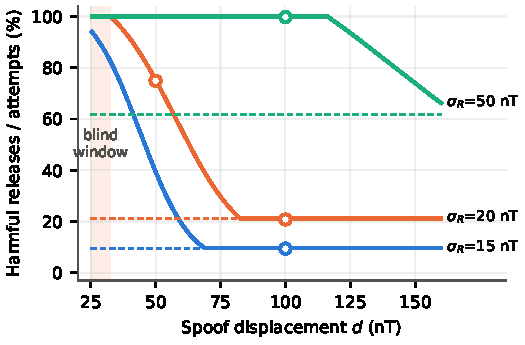
\includegraphics[width=\columnwidth]{figures/reference_theory.pdf}
\caption{Predicted combined-fallback harm versus spoof size (Eq.~\eqref{eq:closed}, median calibrated $\kappa$). Dashed lines: always-reference floor. Circles: confirmation observations with 95\% pipeline intervals. Shaded area: blind window at $\sigma_R=20$~nT. Only the circles are measured.}
\label{fig:theory}
\end{figure}

When hardware independence is compromised, Equation~\eqref{eq:closed} accounts for reference shifts. A $10\text{~nT}$ reference bias increases fallback harm to \ObsBiasHarmRate\%. Partial ($\lambda = 0.5$) and full ($\lambda = 1.0$) coupling result in \HalfHarmRate\% and \FullHarmRate\% harm rates, respectively. In the fully shared case, alarms trigger on only \FullAlarmRate\% of attacks because both primary and reference estimates shift in tandem. A reference sharing the primary sensor's clock generator represents a primary example of such failure modes (Table~\ref{tab:audit}).

\subsection{Post-Hoc Replay: Fusion Trades Worst-Case Integrity for Precision}
\label{sec:results-fusion}

Table~\ref{tab:fusion} evaluates three multi-sensor fusion rules using stored per-attempt primary estimates, reference measurements, and thresholds from the $100\text{~nT}$ and $50\text{~nT}$ spoof scenarios. Rule parameters were established exclusively during clean calibration. The offline replay reproduces frozen fallback counts precisely. While inverse-variance weighting achieves superior clean precision ($\text{RMSE} = \ObsIVWClean\text{~nT}$), it releases harmful estimates on \ObsIVWAttack\% of attacks by heavily weighting the precise yet compromised primary sensor. Soft clipping and gated fusion exhibit intermediate behavior. Across all possible spoof magnitudes, worst-case harm for every rule except standalone reference exceeds $94\%$, corroborating Theorem~\ref{thm:floor}.

\begin{table}[t]
\centering
\caption{Output rules replayed on frozen per-attempt records ($\sigma_R=20$~nT). Gated: reference on alarm, else inverse-variance fusion. Clipped: $R+\mathrm{clip}(\Bhat-R,\pm\kappa)$. Worst case: idealized model maximum over $d\in[0,300]$~nT.}
\label{tab:fusion}
\footnotesize
\setlength{\tabcolsep}{3pt}
\begin{tabular}{@{}lrrrr@{}}
\toprule
& Clean & \multicolumn{2}{c}{Attacked harm (\%)} & Worst \\
Rule & RMSE (nT) & 100~nT & 50~nT & case (\%) \\
\midrule
Always reference & 19.98 & 20.78 & 20.78 & 21.2 \\
Combined fallback & 6.14 & 20.78 & 74.93 & 96.1 \\
Gated fusion & 6.09 & 20.78 & 74.93 & 95.4 \\
Inverse-variance fusion & 4.29 & 100.00 & 100.00 & 100.0 \\
Clipped fusion & 4.38 & 94.86 & 94.86 & 94.9

\\
\bottomrule
\end{tabular}
\end{table}

\subsection{Precision, Availability and Cost}
\label{sec:results-policies}

Table~\ref{tab:policies} summarizes performance across the five pre-registered policies. Combined fallback's primary advantage lies in clean estimation precision ($\text{RMSE} = \FallbackCleanRMSE\text{~nT}$ vs. $\ReferenceCleanRMSE\text{~nT}$ for always-reference, representing a paired improvement of \CleanDifference\text{~nT} $[\CleanDifferenceCI]$, P2). Under attack, fallback's harm matches the reference baseline (P3), while exhibiting higher overall estimation error ($\text{RMSE} = \FallbackAttackRMSE\text{~nT}$ vs. $\ReferenceAttackRMSE\text{~nT}$).

\begin{table*}[t]
\centering
\caption{Nominal case: 100~nT detuning, $\sigma_R=20$~nT, calibrated threshold, \TotalN{} attempts per condition. RMSE is over released outputs. Cost per attempt is modeled primary shots / reference readings; calibration is extra.}
\label{tab:policies}
\small
\setlength{\tabcolsep}{5pt}
\begin{tabular}{@{}lrrrrr@{}}
\toprule
Policy & \shortstack{Clean / attacked\\harmful counts} & \shortstack{Attacked harm\\95\% interval (\%)} & \shortstack{Clean / attacked\\coverage (\%)} & \shortstack{Clean / attacked\\RMSE (nT)} & \shortstack{Shots / reference\\per attempt} \\
\midrule
NLL abstention & 0 / 15{,}194 & [98.73, 99.10] & 98.88 / 98.92 & 4.28 / 100.05 & 20{,}000 / 0 \\
Discrepancy fallback & 144 / 3{,}192 & [20.26, 21.30] & 100.00 / 100.00 & 7.03 / 21.70 & 20{,}000 / 1 \\
Combined abstention & 0 / 296 & [1.71, 2.16] & 98.93 / 1.93 & 4.31 / 97.92 & 20{,}000 / 1 \\
Combined fallback & 88 / 3{,}192 & [20.26, 21.30] & 100.00 / 100.00 & 6.14 / 23.21 & 20{,}000 / 1 \\
Always reference & 3{,}267 / 3{,}192 & [20.26, 21.31] & 100.00 / 100.00 & 19.98 / 19.96 & 0 / 1

\\
\bottomrule
\end{tabular}
\end{table*}

Combined abstention reduces attacked harm by \ObsPFourDiff\text{~pp} compared to fallback (P4), but achieves this solely by suppressing outputs, causing attacked coverage to drop by \ObsPFiveDiff\text{~pp} (P5). In agreement with Corollary~\ref{cor:abstain}, all \AbstainAttackH{} released outputs under attack are harmful (\TheoryAbstainObs\% observed vs. \TheoryAbstainPred\% predicted). Suppressing spoofed estimates incurs a heavy resource penalty, requiring \AbstainShotsMillions{} million primary shots per released estimate under attack. As illustrated in Figure~\ref{fig:curves}, tuning decision thresholds cannot bypass this risk-coverage trade-off. The clean false-alarm rate remains low at \CleanAlarmRate\% $[\CleanAlarmCI]$. Genuine field shifts trigger alarms on only \GenuineAlarmCount{} of \TotalN{} attempts, as both sensors detect the shift simultaneously. Uncalibrated readout drift, however, elevates false alarms to \MismatchAlarmRate\%.

Shot budgets and reference query costs cannot be collapsed into a single metric without platform-specific cost models. However, two general trade-offs apply across implementations:
\begin{enumerate}
\item Combined fallback consumes 20,000 additional primary shots per attempt compared to standalone reference sensing, yielding improved precision under clean conditions as its sole benefit.
\item If reference measurement errors are independent across samples, signal-averaging \TheoryAvgReadings{} reference readings reduces effective noise to $\sigma_R = \TheoryAvgSigma\text{~nT}$—matching fallback's clean RMSE while lowering the worst-case harm floor to \TheoryAvgFloor\%. Consequently, fallback is economically justified only if 20,000 primary shots cost significantly less than \TheoryAvgReadings{} reference queries, or if low-frequency drift ($1/f$ noise) prevents effective reference averaging.
\end{enumerate}

\begin{figure}[t]
\centering
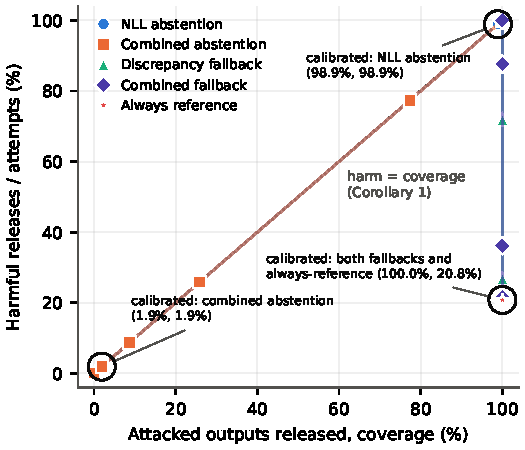
\includegraphics[width=\columnwidth]{figures/confirmation_tradeoffs_column.pdf}
\caption{Frozen threshold family (multipliers 0 to $\infty$) under attack, for 100~nT detuning and $\sigma_R=20$~nT. Rings and labels mark each policy's calibrated point; both fallbacks and always-reference coincide at full coverage. Abstention lies on the diagonal, where harm equals coverage. No operating point is selected from these curves.}
\label{fig:curves}
\end{figure}

% ======================================================================
\section{Discussion}
\label{sec:discussion}

\subsection{Implications for Sensor Design}

Our findings establish four key guidelines for secure quantum sensor design:
\begin{enumerate}
\item \textbf{Match Defenses to Threat Capabilities}: Secret timing offers a computationally lightweight defense against committed phase attacks, but fails completely against frequency detuning.
\item \textbf{Evaluate Recovery, Not Just Detection}: Detection rates provide an incomplete security metric; an anomaly detector can achieve near-perfect detection while still releasing harmful estimates in one out of five attempts.
\item \textbf{Size Reference Precision to Application Tolerances}: By Theorem~\ref{thm:floor}, no translation-equivariant rule can beat the reference floor under worst-case spoofs. Equation~\eqref{eq:kappa} shows that reference noise exceeding $\sigma_R > \TheorySigmaCritical\text{~nT}$ opens a blind window for a $25\text{~nT}$ harm threshold.
\item \textbf{Audit Hardware Dependencies and Leverage Native Structure}: Auxiliary references sharing master clocks, synthesizers, or data paths with the primary sensor offer no true security (Table~\ref{tab:audit}). Conversely, dual-transition protocols algebraically suppress clock manipulation without requiring external hardware, offering a promising target for future experimental demonstration. Similar principles govern Receiver Autonomous Integrity Monitoring (RAIM) in satellite navigation, which decouples fault detection from error exclusion~\cite{brown1992raim,psiaki2016gnss}.
\end{enumerate}

\subsection{Limitations}
\label{sec:limits}

Several constraints define the scope of this study. Simulations model single-transition Ramsey dynamics with ideal pulse envelopes; full spin-1 simulations validate detuning equivalence rather than end-to-end pipeline execution. Experimental confirmation is purely numerical, and physical hardware validation remains necessary. The auxiliary reference is modeled as an abstract Gaussian channel; practical implementations require matched directional alignment, spatial proximity, bandwidth compatibility, and a shared-dependency audit. We evaluate two physical actuation models and finite optimization bounds; adaptive adversaries, multi-actuator co-optimization, or direct reference tampering may expose additional vulnerabilities. Theorem~\ref{thm:floor} applies to translation-equivariant estimators within a location model, leaving prior-aware Bayesian estimation open for further study. Finally, the 30 pipeline replicates evaluate algorithmic and calibration variance across seeds within a single codebase, rather than software implementation diversity. Online recalibration and data poisoning lie outside the current scope.

\subsection{Future Work}

Future work includes evaluating dual-transition sensing protocols under correlated and independent multi-tone attacks, designing specialized fusion rules optimized for the blind window, and validating drive manipulation and reference-assisted verification on physical NV quantum hardware.

% ======================================================================
\section{Related Work}
\label{sec:related}

\textbf{NV Magnetometry.} Ramsey magnetometry with NV centers and its sensitivity limits are well established~\cite{taylor2008magnetometer,rondin2014magnetometry,degen2017quantum,barry2020sensitivity}. Control-robust sequences~\cite{oshnik2022robust} and double-quantum protocols~\cite{fang2013quantumbeats,bauch2018ultralong,hart2021dq} treat control errors as benign imperfections. We treat them as an adversarial capability.

\textbf{Security of Quantum Sensing.} Cryptographic quantum metrology protects quantum resources shared with untrusted parties~\cite{shettell2022cryptographic}. We study the classical control chain of a single sensor.

\textbf{Sensor Spoofing.} Signal injection into analog sensors is well documented~\cite{kune2013ghost,shoukry2013abs}. Physical challenge--response hides probing times to expose spoofers~\cite{shoukry2015pycra}, and fast attackers can bypass timing-based detection~\cite{shin2016sampling}. Our timing result is a Ramsey analogue, but the detuning equivalence defeats challenges entirely rather than winning a speed race. GNSS integrity monitoring likewise separates detection from recovery~\cite{psiaki2016gnss,brown1992raim}.

\textbf{Secure Estimation.} Control theory characterizes undetectable attacks~\cite{pasqualetti2013attack}, designs authentication signals~\cite{mo2009replay} and bounds tolerable corruption~\cite{fawzi2014secure}. Lemma~\ref{lem:equivalence} is an undetectable attack on a quantum sensor, and Proposition~\ref{prop:bound} and Theorem~\ref{thm:floor} are recovery limits for a single trusted auxiliary channel.

\textbf{Calibration and Selective Prediction.} Our thresholds follow the exchangeability argument of conformal prediction~\cite{angelopoulos2023conformal}, and our abstention analysis follows the risk--coverage view of reject options~\cite{chow1970reject,geifman2017selective}.

% ======================================================================

\balance
\section{Conclusion}
\label{sec:conclusion}

A single-transition Ramsey magnetometer cannot distinguish microwave drive detuning from a true magnetic field shift, and secret interrogation timing defends only against committed phase attacks. While an independent reference sensor enables attack detection, it cannot recover field estimates beyond its own inherent accuracy floor. Within a location estimation model, no translation-equivariant fusion rule can bypass this error floor under worst-case spoofing, and small spoofs exploit a critical blind window to evade detection entirely. These theoretical bounds are corroborated by a pre-registered simulation campaign across 30 seeded pipeline replicates and matched by closed-form analytical models. Crucially, these guarantees hold only when the reference sensor is strictly independent of the primary control chain—a condition broken by shared clock sources or synthesizers. For integrity-critical quantum sensing, rigorous reference noise budgeting and hardware dependency audits are far more crucial than raw detection rates, highlighting dual-transition protocols as a vital direction for future research.

\bibliographystyle{IEEEtran}
\bibliography{references}
\end{document}